\section{Auswertung der Messdaten}
\label{sec:Auswertung}

\subsection{Eichung des Magnetfeldes}
\label{sec:magnetfeld}
\begin{table}[H]
    \centering
      \caption{Magnetfeldstärke $B$ für verschiedene Stromstärken $I$.}
      \label{tab:B}
      \sisetup{table-format=3.1}
      \begin{tabular}{S[table-format=1.1] S}
        \toprule
        {$I[\si{\ampere}]$} & {$B[\si{\milli\tesla}]$}\\
        \midrule
        0   &   7.3    \\       
        1   &   106.2  \\
        2   &   206.2  \\
        3   &   301.9  \\
        4   &   388.4  \\
        5   &   462.8  \\
        6   &   522.9  \\
        7   &   560.2  \\
        7.5 &   577.5  \\
        \bottomrule
      \end{tabular}
\end{table}
\noindent

\begin{figure}[H]
    \centering
    \includegraphics[scale= 0.8]{build/magnet.pdf}
    \caption{Magnetfeldstärke $B$ für verschiedene Stromstärken $I$ mit Regression.}
    \label{fig:B}
\end{figure}
\noindent

\begin{align*}
    a&=\SI{-0.59\pm 0.06}{\milli\tesla\per\cubic\ampere}\\
    b&=\SI{1.20 \pm 0.66}{\milli\tesla\per\square\ampere}\\
    c&=\SI{99.91\pm 2.05}{\milli\tesla\per\ampere}\\
    d&=\SI{6.68 \pm 1.64}{\milli\tesla}
\end{align*}

\subsection{Auswertung der roten Spektrallinie}
\label{sec:rot}

\begin{figure}[H]
    \centering
    
\includegraphics[scale= 0.2]{Messung/Rot[6].JPG}
    \caption{Interferenzmuster der roten Spektrallinie ohne Magnetfeld.}
    \label{fig:rot}
\end{figure}
\noindent

\begin{figure}[H]
    \centering
    
\includegraphics[scale= 0.2]{Messung/Rot_Sigma[7].JPG}
    \caption{Interferenzmuster der roten Spektrallinie beim $\sigma$-Übergang.}
    \label{fig:rot_sigma}
\end{figure}
\noindent

\begin{table}[H]
    \centering
      \caption{Messwerte für die Linienabstände $\Delta s$ und die Aufspaltung $\delta s$ in Pixeln für die rote Spektrallinie.}
      \label{tab:rot}
      \sisetup{table-format=3.1}
      \begin{tabular}{S[table-format=1.1] S}
        \toprule
        {$\Delta s[\text{px}]$} & {$\delta s[\text{px}]$}\\
        \midrule
        117.9  &  59.2 \\
        128.2  &  56.0 \\
        134.4  &  53.3 \\
        144.6  &  55.1 \\
        149.8  &  63.3 \\
        160.6  &  72.0 \\
        178.7  &  74.7 \\
        202.4  &  84.9 \\
        \bottomrule
      \end{tabular}
\end{table}
\noindent

\begin{align*}
    \overline{\Delta s}&=\num{152.1\pm 26.0}\text{px}\\
    \overline{\delta s}&=\num{64.81\pm 64.8}\text{px}
\end{align*}

\subsection{Auswertung der blauen Spektrallinie}
\label{sec:blau}
\begin{figure}[H]
    \centering
    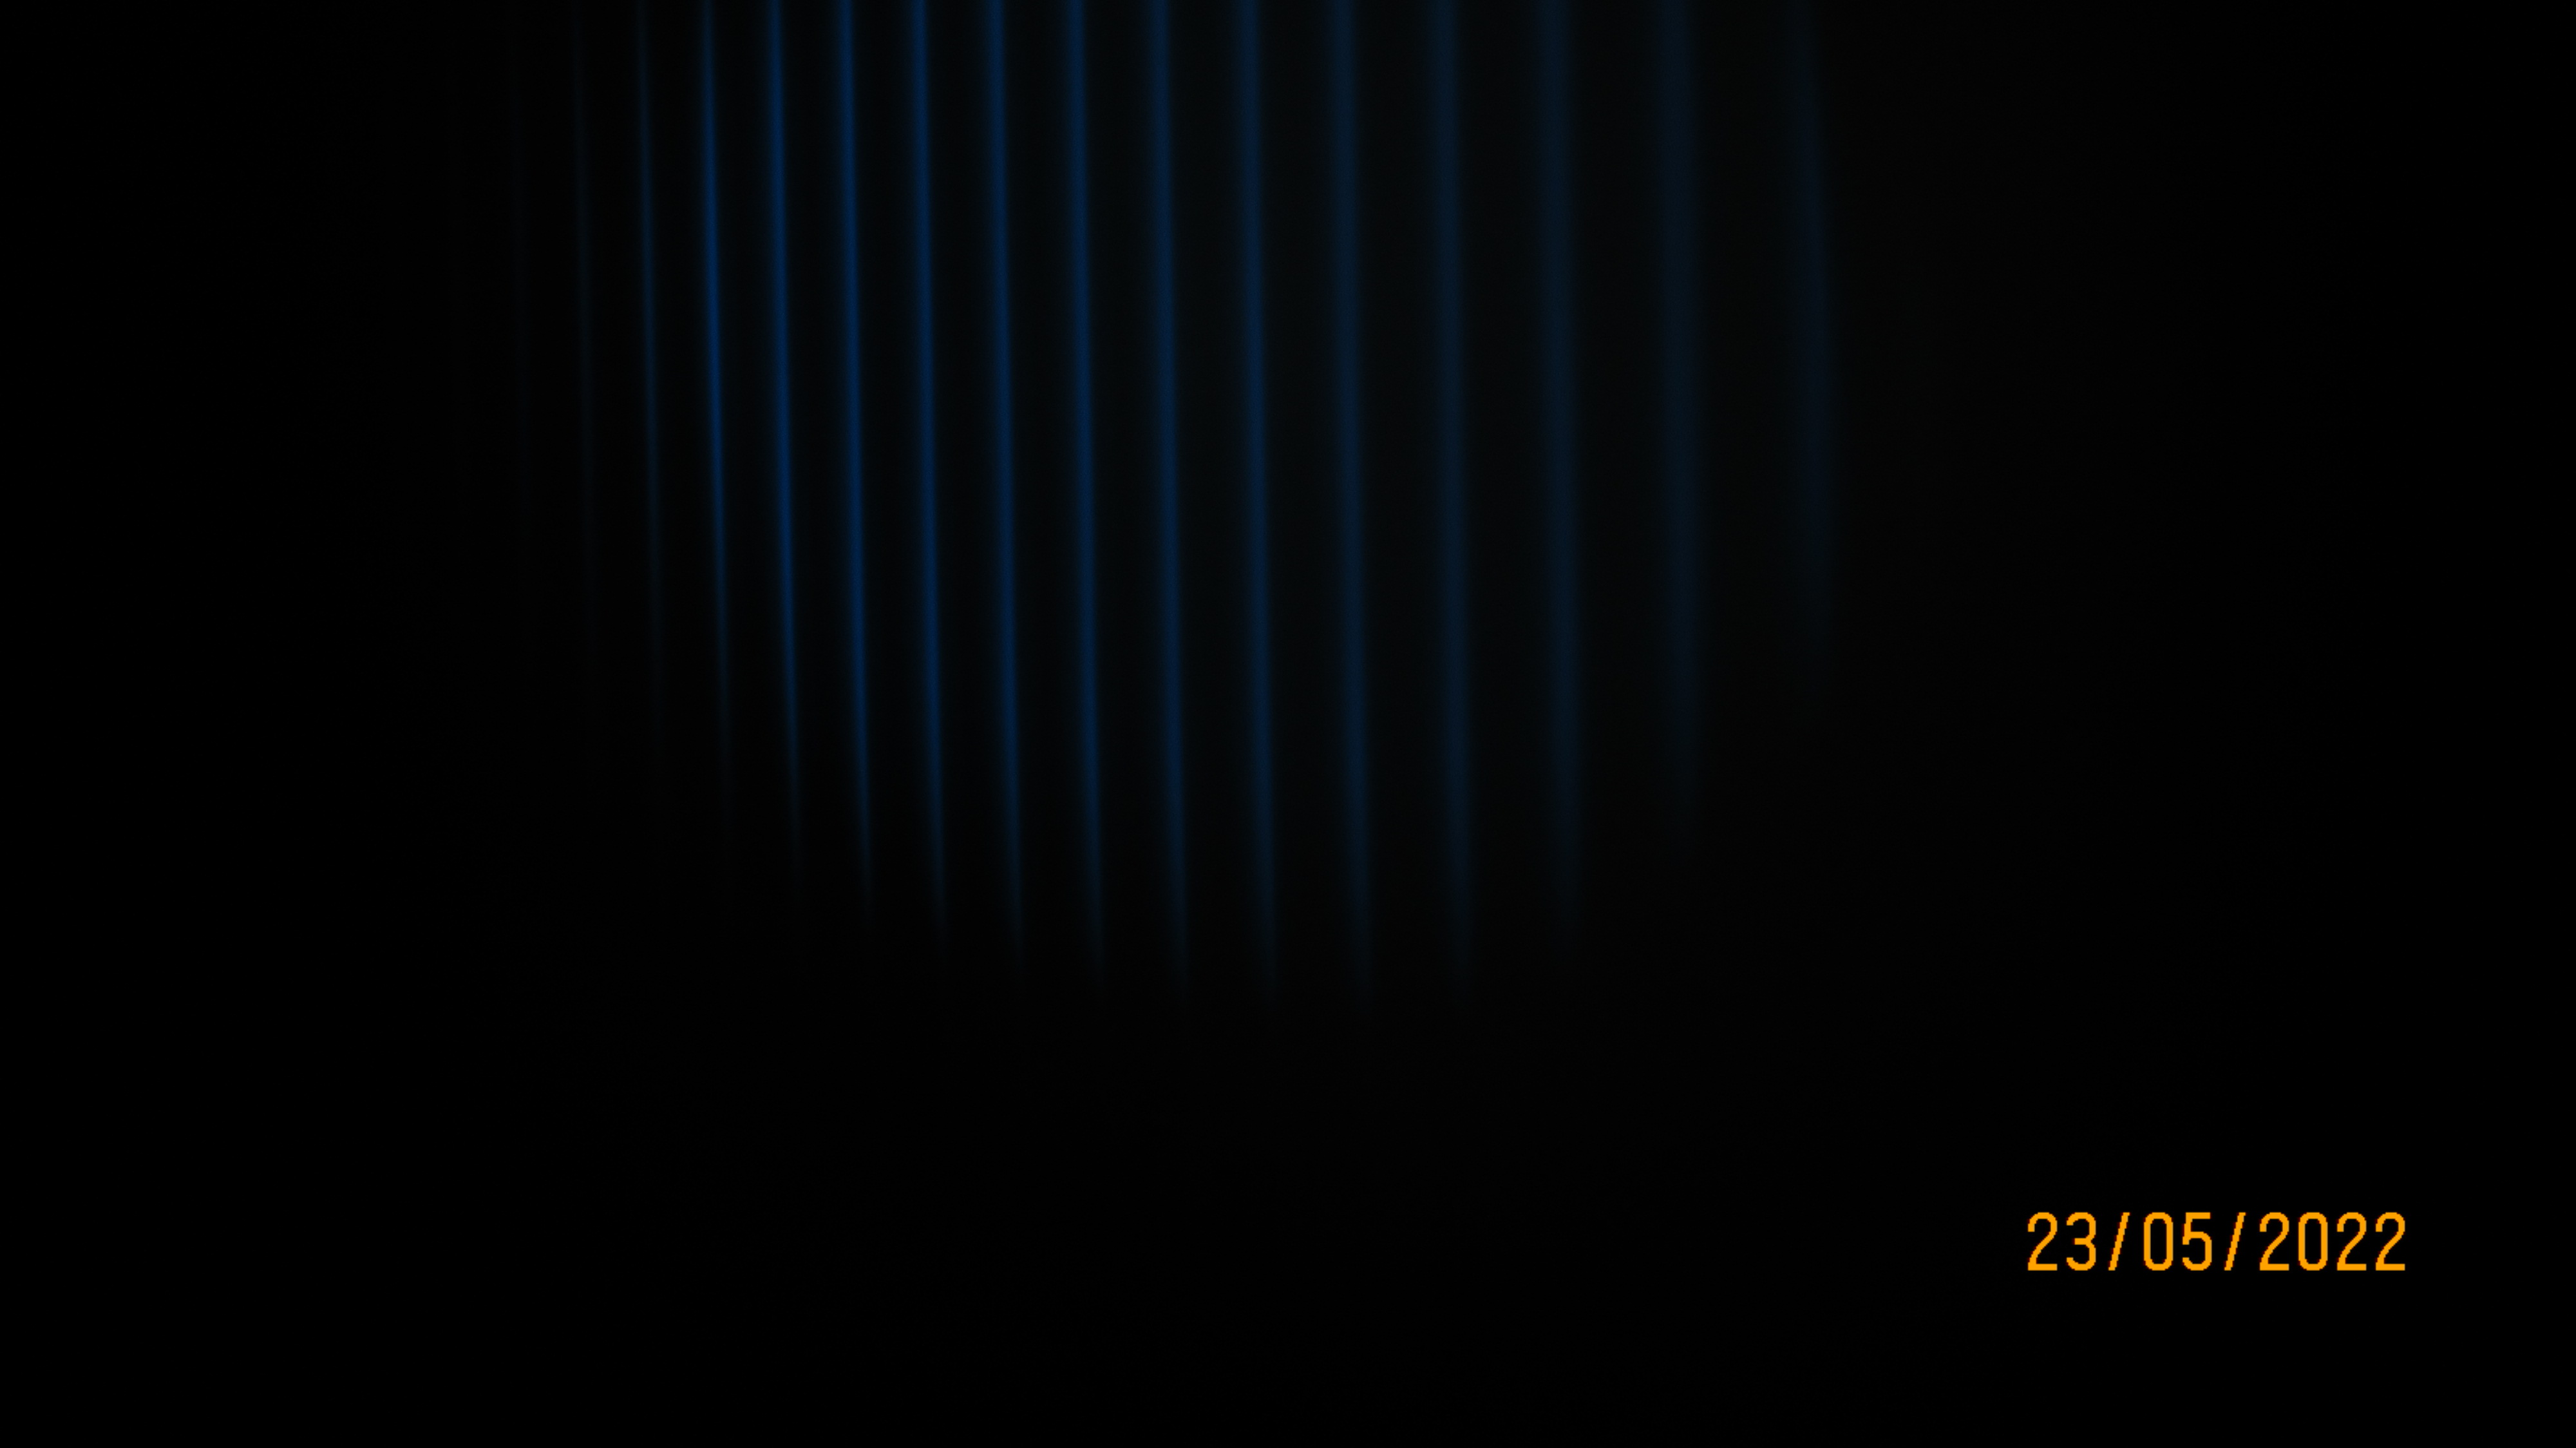
\includegraphics[scale= 0.2]{Messung/Blau[3].JPG}
    \caption{Interferenzmuster der blauen Spektrallinie ohne Magnetfeld.}
    \label{fig:blau}
\end{figure}
\noindent


\subsubsection[]{$\sigma$-Übergang}
\label{sec:sigma}

\begin{figure}[H]
    \centering
    
\includegraphics[scale= 0.2]{Messung/Blau_Sigma[4].JPG}
    \caption{Interferenzmuster der blauen Spektrallinie beim $\sigma$-Übergang.}
    \label{fig:blau_sigma}
\end{figure}
\noindent

\begin{table}[H]
    \centering
      \caption{Messwerte für die Linienabstände $\Delta s$ und die Aufspaltung $\delta s$ in Pixeln für dden $\sigma$-Übergang der blaue Spektrallinie.}
      \label{tab:blau_sigma}
      \sisetup{table-format=3.1}
      \begin{tabular}{S[table-format=1.1] S}
        \toprule
        {$\Delta s[\text{px}]$} & {$\delta s[\text{px}]$}\\
        \midrule
        84.4  &  30.0 \\
        92.0  &  33.5 \\
        96.8  &  37.0 \\
        99.0  &  38.2 \\
        104.4 &  40.5 \\
        108.0 &  41.8 \\
        114.0 &  44.5 \\
        118.0 &  41.5 \\
        131.0 &  44.4 \\
        140.7 &  47.9 \\
        147.1 &  53.3 \\
        166.0 &  53.2 \\
        190.6 &  55.1 \\
        \bottomrule
      \end{tabular}
\end{table}
\noindent

\begin{align*}
    \overline{\Delta s}&=\num{122.5\pm 30.1}\text{px}\\
    \overline{\delta s}&=\num{43.2\pm 7.4}\text{px}
\end{align*}


\subsubsection[]{$\pi$-Übergang}
\label{sec:pi}

\begin{figure}[H]
    \centering
    
\includegraphics[scale= 0.2]{Messung/Blau_Pi[5].JPG}
    \caption{Interferenzmuster der blauen Spektrallinie beim $\pi$-Übergang.}
    \label{fig:blau_pi}
\end{figure}
\noindent

\begin{table}[H]
    \centering
      \caption{Messwerte für die Linienabstände $\Delta s$ und die Aufspaltung $\delta s$ in Pixeln für den $\pi$-Übergang der blaue Spektrallinie.}
      \label{tab:blau_pi}
      \sisetup{table-format=3.1}
      \begin{tabular}{S[table-format=1.1] S}
        \toprule
        {$\Delta s[\text{px}]$} & {$\delta s[\text{px}]$}\\
        \midrule
        84.4  &  30.0 \\
        92.0  &  33.5 \\
        96.8  &  37.0 \\
        99.0  &  38.2 \\
        104.4 &  40.5 \\
        108.0 &  41.8 \\
        114.0 &  44.5 \\
        118.0 &  41.5 \\
        131.0 &  44.4 \\
        140.7 &  47.9 \\
        147.1 &  53.3 \\
        166.0 &  53.2 \\
        190.6 &  55.1 \\
        \bottomrule
      \end{tabular}
\end{table}
\noindent

\begin{align*}
    \overline{\Delta s}&=\num{122.5\pm 30.1}\text{px}\\
    \overline{\delta s}&=\num{33.6 \pm 10.5}\text{px}
\end{align*}
